\documentclass{article}

\usepackage{fancyhdr}
\usepackage{extramarks}
\usepackage{amsmath}
\usepackage{amsthm}
\usepackage{amsfonts}
\usepackage{tikz}
\usepackage{enumerate}
\usepackage{graphicx}
\graphicspath{ {images/} }
\usepackage[plain]{algorithm}
\usepackage{algpseudocode}
\usepackage[document]{ragged2e}
\usepackage{textcomp}
\usepackage{color}   %May be necessary if you want to color links
\usepackage{hyperref}
\hypersetup{
    colorlinks=true, %set true if you want colored links
    linktoc=all,     %set to all if you want both sections and subsections linked
    linkcolor=black,  %choose some color if you want links to stand out
}

\usetikzlibrary{automata,positioning}

%
% Basic Document Settings
%

\topmargin=-0.45in
\evensidemargin=0in
\oddsidemargin=0in
\textwidth=6.5in
\textheight=9.0in
\headsep=0.25in
\setlength{\parskip}{1em}

\linespread{1.1}

\pagestyle{fancy}
\lhead{\hmwkAuthorName}
%\chead (\hmwkTitle}
%\rhead{\firstxmark}
\lfoot{\lastxmark}
\cfoot{\thepage}

\renewcommand\headrulewidth{0.4pt}
\renewcommand\footrulewidth{0.4pt}

\setlength\parindent{0pt}

%
% Create Problem Sections
%

\newcommand{\enterProblemHeader}[1]{
    \nobreak\extramarks{}{Question \arabic{#1} continued on next page\ldots}\nobreak{}
    \nobreak\extramarks{Question \arabic{#1} (cont.)}{Question \arabic{#1} continued on next page\ldots}\nobreak{}
}

\newcommand{\exitProblemHeader}[1]{
    \nobreak\extramarks{Question \arabic{#1} (cont.)}{Question \arabic{#1} continued on next page\ldots}\nobreak{}
    \stepcounter{#1}
    \nobreak\extramarks{Question \arabic{#1}}{}\nobreak{}
}

\setcounter{secnumdepth}{0}
\newcounter{partCounter}
\newcounter{homeworkProblemCounter}
\setcounter{homeworkProblemCounter}{1}
\nobreak\extramarks{Problem \arabic{homeworkProblemCounter}}{}\nobreak{}

%
% Homework Problem Environment
%
% This environment takes an optional argument. When given, it will adjust the
% problem counter. This is useful for when the problems given for your
% assignment aren't sequential. See the last 3 problems of this template for an
% example.
%
\newenvironment{homeworkProblem}[1][-1]{
    \ifnum#1>0
        \setcounter{homeworkProblemCounter}{#1}
    \fi
    \section{Problem \arabic{homeworkProblemCounter}}
    \setcounter{partCounter}{1}
    \enterProblemHeader{homeworkProblemCounter}
}{
    \exitProblemHeader{homeworkProblemCounter}
}

%
% Homework Details
%   - Title
%   - Due date
%   - Class
%   - Section/Time
%   - Instructor
%   - Author
%

\newcommand{\hmwkTitle}{Math GRE Subject Test Notes}
%%\newcommand{\hmwkDueDate}{September 14, 2017}
%\newcommand{\hmwkClass}{Math 4650}
%\newcommand{\hmwkClassTime}{Section A}
%\newcommand{\hmwkClassInstructor}{A. Shaheen}
\newcommand{\hmwkAuthorName}{\textbf{G. Faletto} }

%
% Title Page
%

\title{
    \vspace{2in}
    \textmd{\textbf{ \hmwkTitle}}\\
%    \normalsize\vspace{0.1in}\small{Due\ on\ \hmwkDueDate}\\
%    \vspace{0.1in}\large{\textit{Instructor: Tony Shaheen\ }}
%    \vspace{3in}
}

\author{Gregory Faletto}
\date{}

\renewcommand{\part}[1]{\textbf{\large Part \Alph{partCounter}}\stepcounter{partCounter}\\}

%
% Various Helper Commands
%

% Useful for algorithms
\newcommand{\alg}[1]{\textsc{\bfseries \footnotesize #1}}

% For derivatives
\newcommand{\deriv}[2]{\frac{\mathrm{d} #1}{\mathrm{d} #2}}

% For partial derivatives
\newcommand{\pderiv}[2]{\frac{\partial #1}{\partial #2}}

% Integral dx
\newcommand{\dx}{\mathrm{d}x}

% Alias for the Solution section header
\newcommand{\solution}{\textbf{\large Solution}}

% Probability commands: Expectation, Variance, Covariance, Bias
\newcommand{\E}{\mathbb{E}}
\newcommand{\Var}{\mathrm{Var}}
\newcommand{\Cov}{\mathrm{Cov}}
\newcommand{\Bias}{\mathrm{Bias}}

% Tilde
\newcommand{\textapprox}{\raisebox{0.5ex}{\texttildelow}}

\begin{document}

\maketitle

\pagebreak

\tableofcontents

\newpage

% Linear Algebra
\section{Linear Algebra}
\subsection{Properties of Projection Matrices}

\begin{enumerate}[i.]

\item Formula:

\[
P = A(A^TA)^{-1}A^T
\]

(Note that if \(A\) is an invertible (square) matrix, then \(P = A(A^TA)^{-1}A^T = AA^{-1}(A^T)^{-1}A^T = I\).)

\textbf{The projection matrix projects any vector \(b\) into the column space of \(A\).} In other words, \(p = Pb\) is the component of \(b\) in the column space, and the error \(e = b - Pb\) is the component in the orthogonal complement. (\(I - P\) is also a projection matrix. It projects \(b\) onto the orthogonal complement, and the projection is \(b - Pb = e\)).

(Note that if \(A\) is an invertible (square) matrix, then its column space is all of \(\mathbb{R}^n\), so \(b\) is already in the column space of \(A\).)

\item The projection matrix is \textbf{idempotent}: it equals its square--\(P^2 = P\).

\item The projection matrix is \textbf{symmetric}: it equals its transpose--\(P^T = P\).

\item Conversely, \textbf{any symmetric idempotent matrix represents a projection}. \(P\) is unique for a given subspace.

\item If \(A\) is an \(m \times n\) matrix with rank \(n\), then \(\text{rank} (P) = n\). The eigenvalues of \(P\) consist of \(n\) ones and \(m - n\) zeroes. \(P\) always contains \(n\) independent eigenvectors and is thus diagonalizable. 

\end{enumerate}

Suppose \(A\) is a square nonsingular matrix and \(\lambda\) is an eigenvalue of \(A\). Then \(\lambda^{-1}\) is an eigenvalue of the matrix \(A^{-1}\).

\subsection{Eigenvalues, Eigenvectors, Diagonalization, Symmetric Matrices}

\textbf{Notes on Diagonalization}

Suppose the \(n \times n\) matrix \(A\) has \(n\) linearly independent eigenvectors. If these eigenvectors are the columns of a matrix \(S\), then \(S^{-1}AS\) is a diagonal matrix \(\Lambda\). The eigenvalues of \(A\) are on the diagonal of \(\Lambda\):

\[
S^{-1}AS = \Lambda = \begin{bmatrix}
   \lambda_1       & 0  & \cdots  & 0  \\
  0  & \lambda_2 & \cdots  & 0 \\
  \vdots  & \vdots  & \ddots & \vdots \\
   0  & 0 & \cdots & \lambda_n
\end{bmatrix}
\]

We call \(S\) the \textbf{eigenvector matrix} and \(\Lambda\) the \textbf{eigenvalue matrix}.

\begin{enumerate}[1.]

\item If the matrix \(A\) has no repeated eigenvalues, then its \(n\) eigenvectors are automatically independent. Therefore \textbf{any matrix with \(n\) distinct eigenvalues can be diagonalized}.

\item \textbf{The diagonalizing matrix \(S\) is not unique}. An eigenvector \(x\) can be multiplied by a constant and remains an eigenvector. We can multiply the columns of \(S\) by any nonzero constants and produce a new diagonalizing \(S\). Repeated eigenvalues leave even more freedom in \(S\) (columns with identical eigenvalues can be interchanged). 

(Note that for the trivial example \(A = I\), any invertible \(S\) will do. \(S^{-1}IS\) is always diagonal, and \(\Lambda\) is just \(I\). \textbf{All vectors are eigenvectors of the identity.})

\item \textbf{Other matrices \(S\) will not produce a diagonal \(\Lambda\)}. Since \(\Lambda = S^{-1}AS\), \(S\) must satisfy \(S \Lambda = AS\). Suppose the first column of \(S\) is \(y\). Then the first column of \(S \Lambda\) is \(\lambda_1y\). If this is to agree with the first column of \(AS\), which by matrix multiplication is \(Ay\), then \(y\) must be an eigenvector: \(Ay = \lambda_1y\). 

(Note that the \textit{order} of the eigenvectors in \(S\) and the eigenvalues in \(\Lambda\) must match.)

\item Not all matrices posses \(n\) linearly independent eigenvectors, so \textbf{not all matrices are diagonalizable}. 

\textbf{Diagonalizability of \(A\) depends on having enough (\(n\)) independent eigenvectors. Invertibility of \(A\) depends on having nonzero eigenvalues.}

There is no connection between diagonalizability (\(n\) independent eigenvectors) and invertibility (no zero eigenvalues). The only indication given by the eigenvalues is that diagonalization can fail only if there are repeated eigenvalues. (But even then, it does not always fail--e.g. \(I\).)

The test is to check, for an eigenvalue that is repeated \(p\) times, whether there are \(p\) independent eigenvectors--in other words, whether \(A - \lambda\) has rank \(n - p\).

%If eigenvectors \(x_1, x_2, \ldots, x_k\) correspond to different eigenvalues \(\lambda_1, \lambda_2, \ldots, \lambda_k\), then those eigenvectors are linearly independent.

\item \textbf{Projection matrices always contain \(n\) independent eigenvectors and thus are always diagonalizable}.

\end{enumerate}

\textbf{Eigenvalues of Symmetric Matrices:} If \(A\) is symmetric, then it has the following properties:

\begin{enumerate}[1.]

\item \(A\) has exactly \(n\) (not necessarily distinct) eigenvalues

\item There exists a set of \(n\) eigenvectors, one for each eigenvalue, that are mutually orthogonal (even if the eigenvalues are not distinct).

\end{enumerate}

\textbf{Eigenvalues of the Inverse of a Matrix:} Suppose \(A\) is a square nonsingular matrix and \(\lambda\) is an eigenvalue of \(A\). Then \(\lambda^{-1}\) is an eigenvalue of the matrix \(A^{-1}\). Proof: Note that since \(A\) is nonsingular, \(A^{-1}\) exists and \(\lambda\) is nonnegative for all eigenvalues of \(A\). Let \(\lambda\) be an eigenvalue of \(A\) and let \(x \neq 0\) be an eigenvector of \(A\) for \(\lambda\). Suppose \(A\) is \(n\) by \(n\). Then we have

\[
A^{-1}x = A^{-1}\lambda^{-1} \lambda x = \lambda^{-1} A^{-1} \lambda x = \lambda^{-1} A^{-1} A x = \lambda^{-1}x
\]

\textbf{The inverse of a symmetric matrix is symmetric.} Proof: Let \(A\) be a symmetric matrix.

\[
I = I'
\]

\[
A A^{-1} = (A A^{-1})'
\]

\[
A^{-1} A = (A^{-1})'A'
\]

\[
A^{-1} A A^{-1} = (A^{-1})'A A^{-1}
\]

\[
A^{-1} = (A^{-1})'
\]

\subsection{Positive Definite Matrices}

For any real invertible matrix \(A\), the product \(A' A\) is a positive definite matrix. (Proof: Let \(z\) be a non-zero vector. We want \(z' A' A z >0 \forall z\). Note that \(z' A' A z = (Az)'(Az)\). Because \(A\) is invertible and \(z \neq 0\), \(Az \neq 0 \), so \((Az)'(Az) > 0\).)

Let \(A \in \mathbb{R}^{m \times n}\) with \(m \geq n\) and let \(\text{rank}(A) = n\) (that is, \(A\) has full column rank). Then \(A' A\) is a positive definite matrix. (Proof: Let \(z\) be a non-zero vector. We want \(z' A' A z >0 \forall z\). Note that \(z' A' A z = (Az)'(Az)\). Because \(A\) has full column rank (and \(n\) linearly independent columns) and \(z \neq 0\), \(Az \neq 0 \), so \((Az)'(Az) > 0\).)

Every positive definite matrix is invertible and its inverse is also positive definite.

\subsection{Practice Problems}

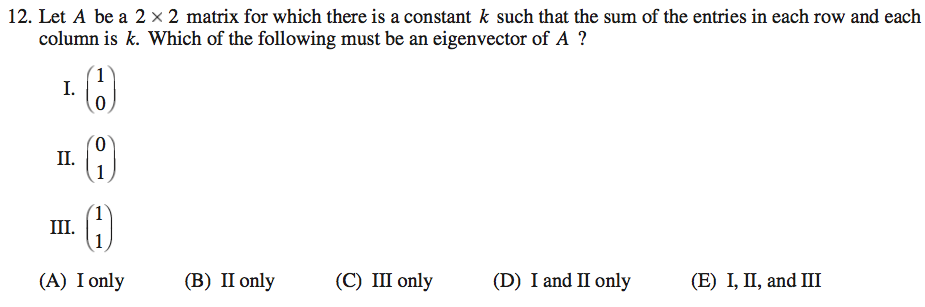
\includegraphics[scale=0.5]{0568_12}

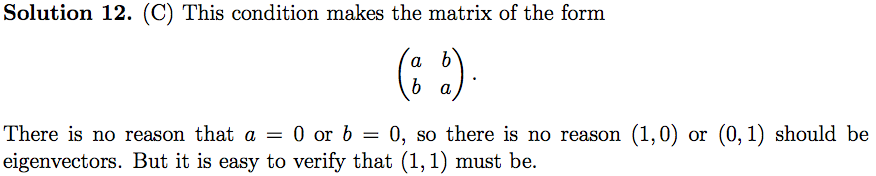
\includegraphics[scale=0.5]{0568_12s}

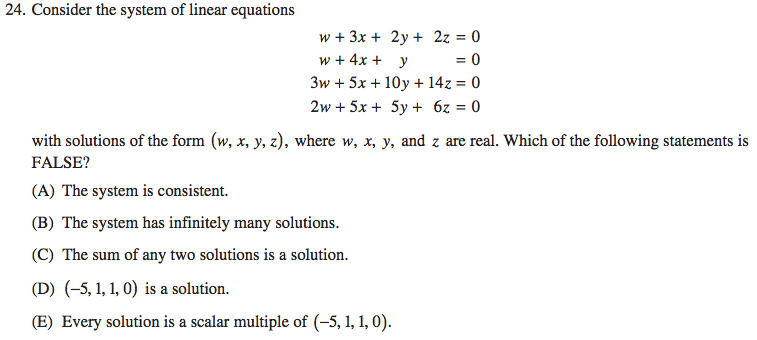
\includegraphics[scale=0.65]{1268_24}

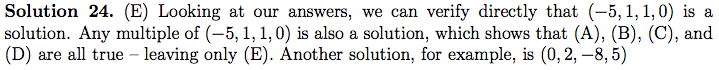
\includegraphics[scale=0.65]{1268_24s}

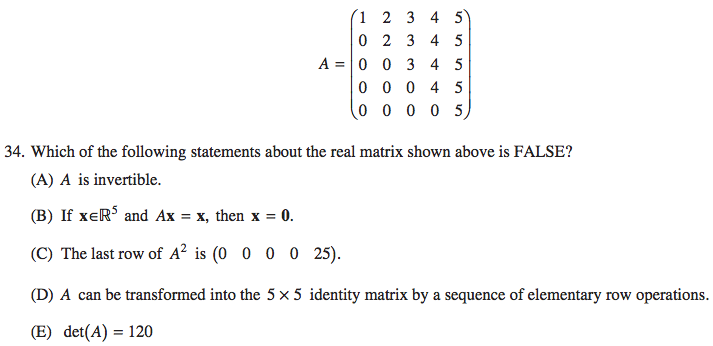
\includegraphics[scale=0.65]{1268_34}

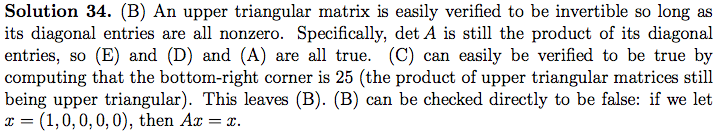
\includegraphics[scale=0.65]{1268_34s}

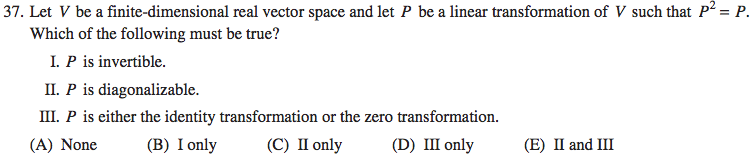
\includegraphics[scale=0.65]{1268_37}

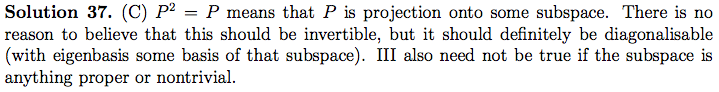
\includegraphics[scale=0.65]{1268_37s}

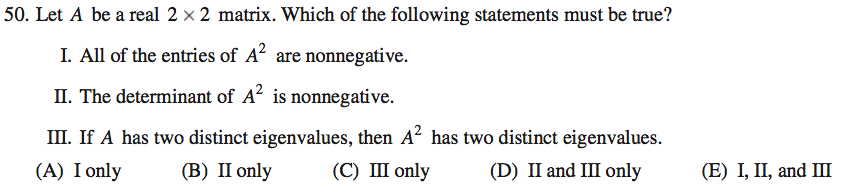
\includegraphics[scale=0.5]{0568_50}

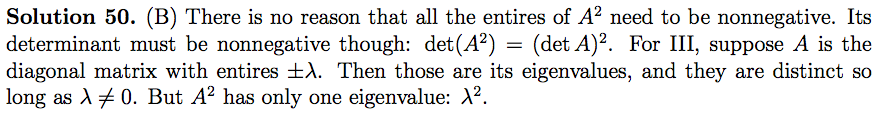
\includegraphics[scale=0.5]{0568_50s}

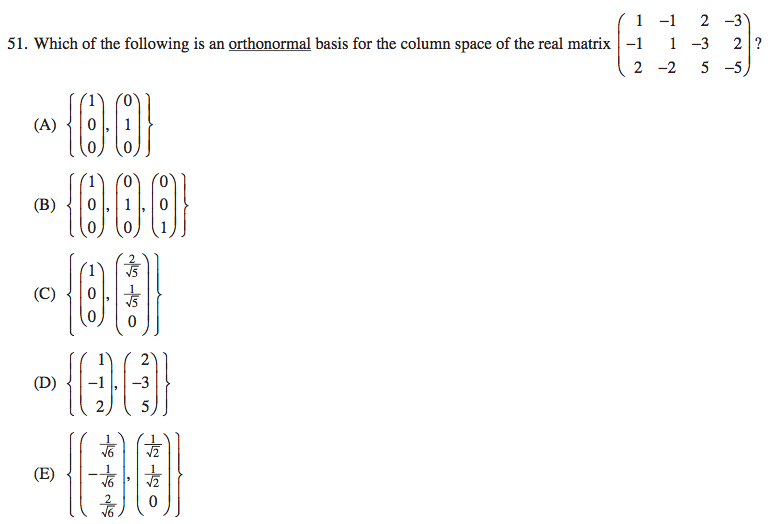
\includegraphics[scale=0.65]{1268_51}

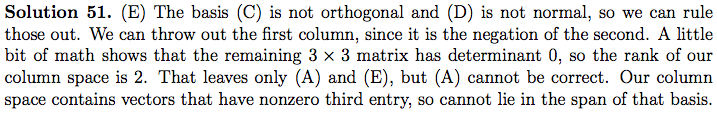
\includegraphics[scale=0.65]{1268_51s}

%%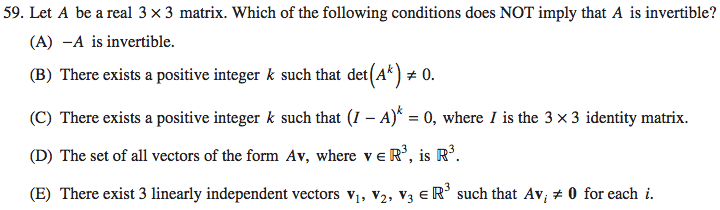
\includegraphics[scale=0.65]{1268_59}
%
%%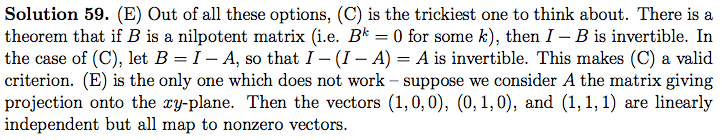
\includegraphics[scale=0.65]{1268_59s}

\pagebreak

% Calculus
\section{Calculus}

\subsection{List of common derivatives and integrals to know}

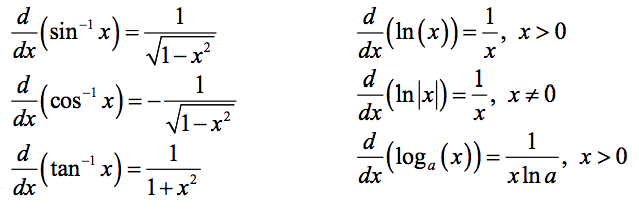
\includegraphics[scale=0.45]{derivatives}

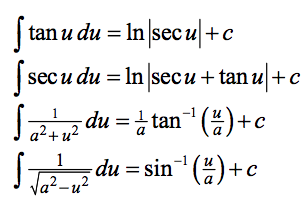
\includegraphics[scale=0.45]{integrals}

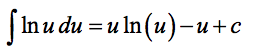
\includegraphics[scale=0.45]{integral_ln}

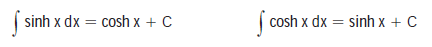
\includegraphics[scale=0.65]{integrals2}

\subsection{Optimizing functions of several variables}

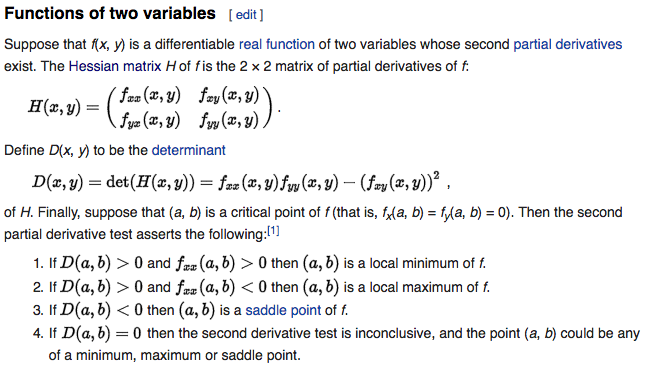
\includegraphics[scale=0.65]{hessian1}

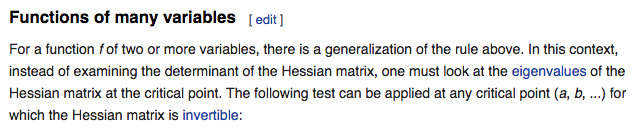
\includegraphics[scale=0.65]{hessian2}

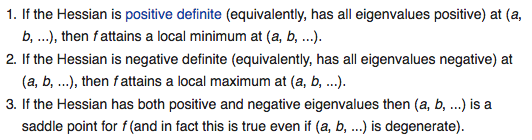
\includegraphics[scale=0.65]{hessian3}

\subsection{Lagrange Multipliers} \textbf{: to flesh out!} http://tutorial.math.lamar.edu/Classes/CalcIII/LagrangeMultipliers.aspx

\subsection{Line Integrals} (p. 555 of Strang book)

Suppose a force in two-dimensional space is given by \(\boldsymbol{F} = M\boldsymbol{i} + N \boldsymbol{j}\). Then the work done by this force on a particle moving along a curve \(C\) is given by

\[
W = \int_C \boldsymbol{F} \cdot \text{d}\boldsymbol{R} = \int_C M \text{d}x + N \text{d} y
\]

Along a curve in three-dimensional space the work done by a three-dimensional force \(\boldsymbol{F} = M\boldsymbol{i} + N \boldsymbol{j} + P \boldsymbol{j}\) is given by

\[
W = \int_C \boldsymbol{F} \cdot \boldsymbol{T} \text{d}s = \int_C \boldsymbol{F} \cdot \text{d}\boldsymbol{R} = \int_C M \text{d}x + N \text{d}y + P \text{d}z
\]

where the tangent vector \(\boldsymbol{T}\) is given by \[\boldsymbol{T} = \frac{\text{d}\boldsymbol{R}}{\text{d}s}\]

\textbf{Green's Theorem:} Suppose the region \(R\) is bounded by the simple closed piecewise smooth curve \(C\). Then an integral over \(R\) equals a line integral around \(C\):

\[
\oint_C \boldsymbol{F} \cdot \text{d}\boldsymbol{R} = \oint_C M \text{d}x + N \text{d}y = \int \int_R \bigg( \frac{\partial N}{\partial x} - \frac{\partial M}{\partial y} \bigg) \text{d}x \ \text{d}y
\]

\subsection{Miscellaneous}

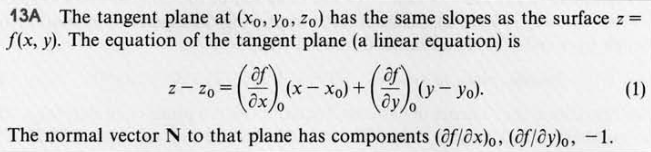
\includegraphics[scale=0.65]{tangent_plane}

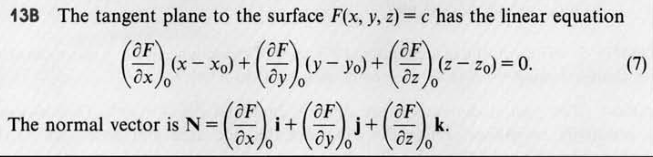
\includegraphics[scale=0.65]{tangent_plane2}

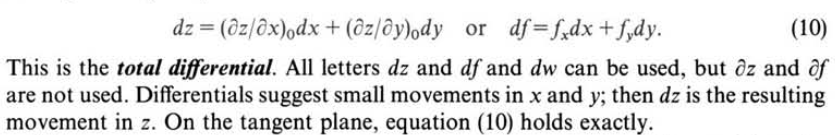
\includegraphics[scale=0.55]{total_differential}

The \textbf{directional derivative}, denoted \(D_v f(x, y)\), is a derivative of a multivariable function in the direction of a vector \(\boldsymbol{v}\). It is the scalar projection of the gradient onto \(\boldsymbol{v}\).

\[
D_v f(x, y) = \text{comp}_v \nabla f(x, y) = \frac{\nabla f(x, y) \cdot \boldsymbol{v}}{|\boldsymbol{v}|}
\]

\subsection{Practice Problems}

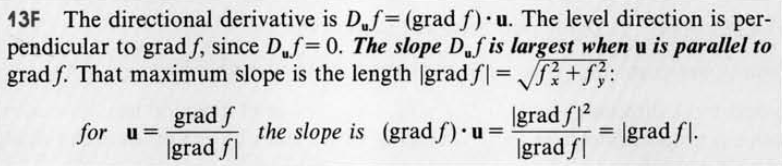
\includegraphics[scale=0.55]{gradient}

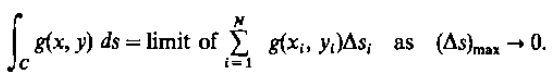
\includegraphics[scale=0.55]{line_int1}

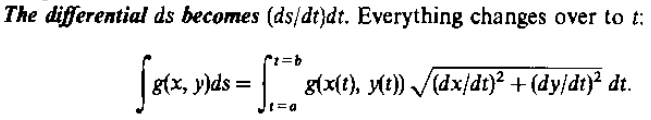
\includegraphics[scale=0.55]{line_int2}

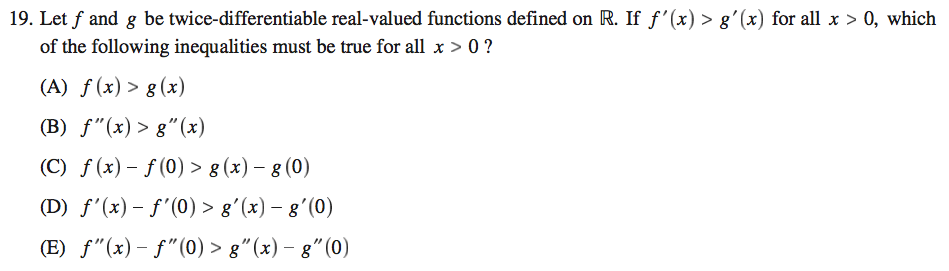
\includegraphics[scale=0.5]{0568_19}

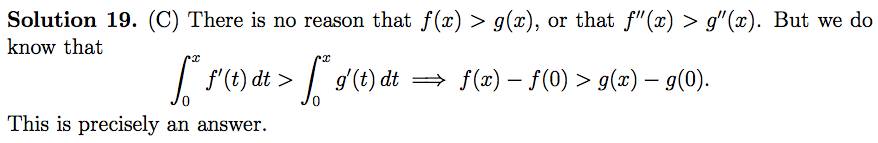
\includegraphics[scale=0.5]{0568_19s}

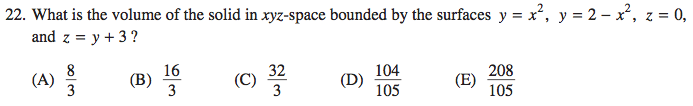
\includegraphics[scale=0.65]{1268_22}

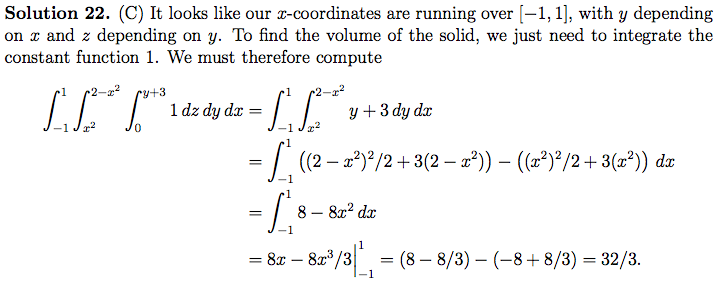
\includegraphics[scale=0.65]{1268_22s}

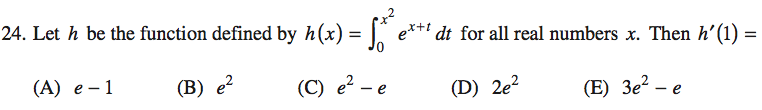
\includegraphics[scale=0.5]{0568_24}

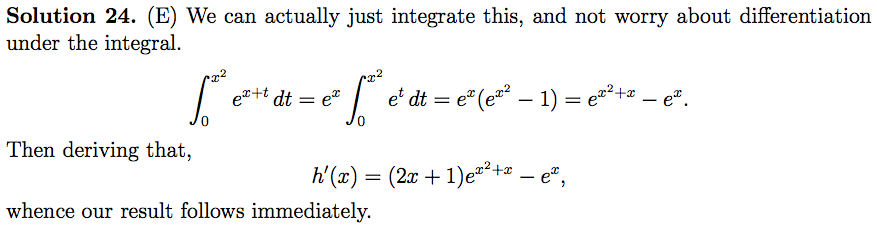
\includegraphics[scale=0.5]{0568_24s}

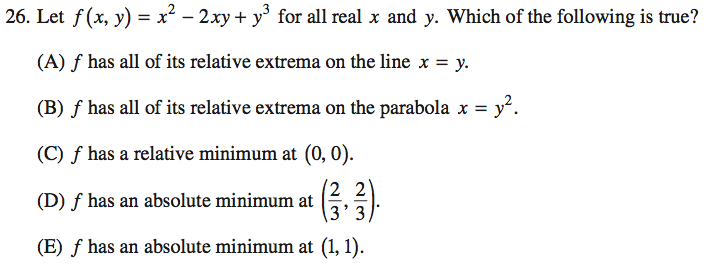
\includegraphics[scale=0.5]{0568_26}

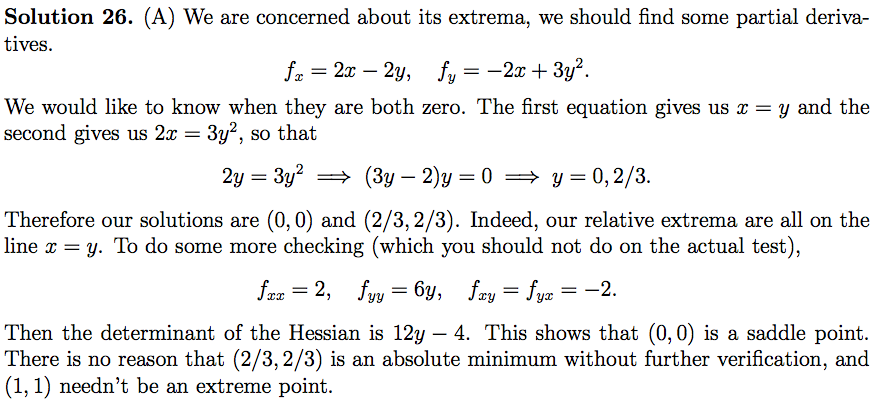
\includegraphics[scale=0.5]{0568_26s}

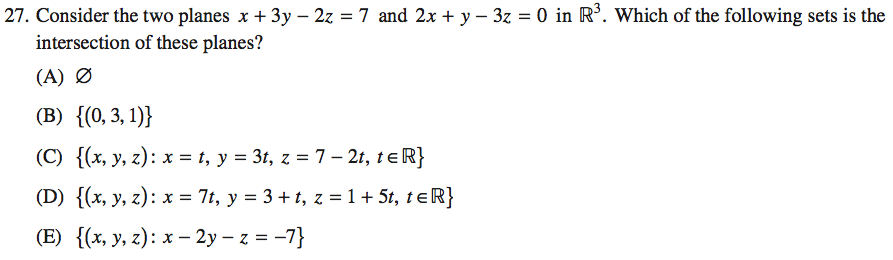
\includegraphics[scale=0.5]{0568_27}

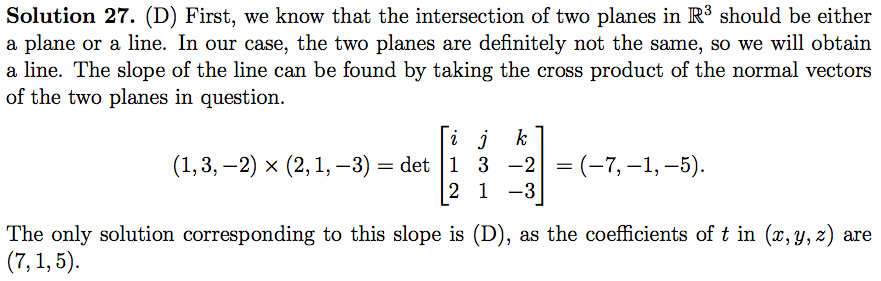
\includegraphics[scale=0.5]{0568_27s}

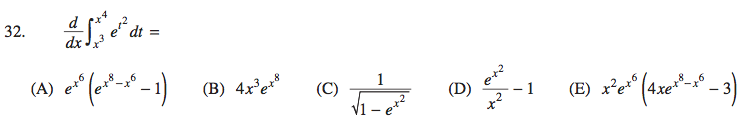
\includegraphics[scale=0.65]{1268_32}

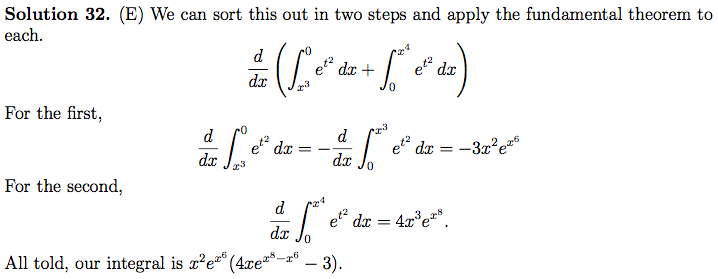
\includegraphics[scale=0.65]{1268_32s}

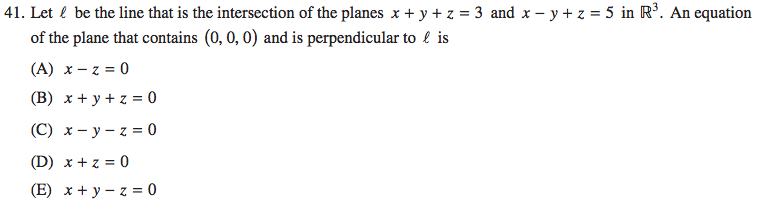
\includegraphics[scale=0.65]{1268_41}

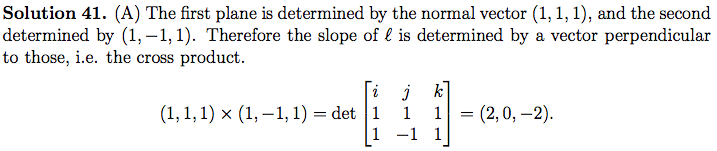
\includegraphics[scale=0.65]{1268_41s1}

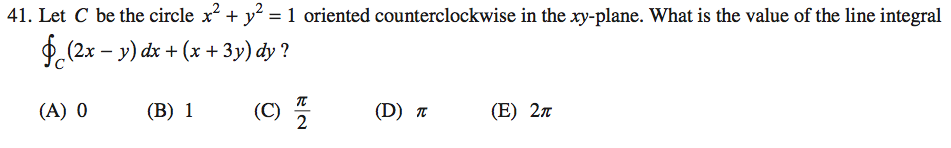
\includegraphics[scale=0.5]{0568_41}

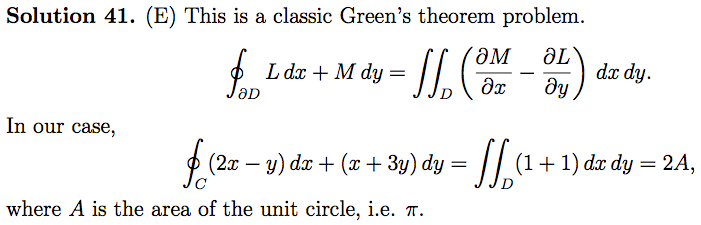
\includegraphics[scale=0.5]{0568_41s}

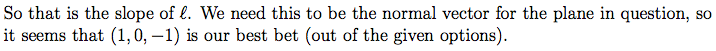
\includegraphics[scale=0.65]{1268_41s2}

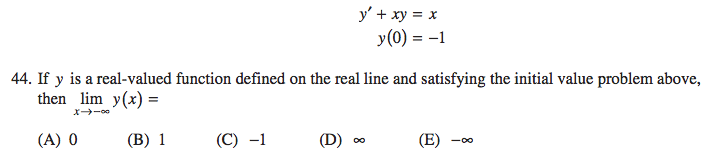
\includegraphics[scale=0.65]{1268_44}

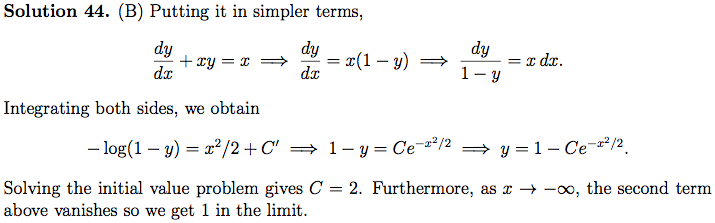
\includegraphics[scale=0.65]{1268_44s}


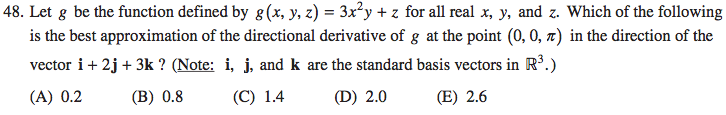
\includegraphics[scale=0.65]{1268_48}

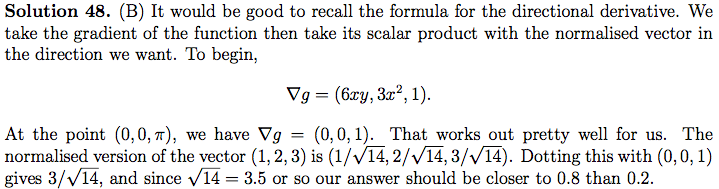
\includegraphics[scale=0.65]{1268_48s}

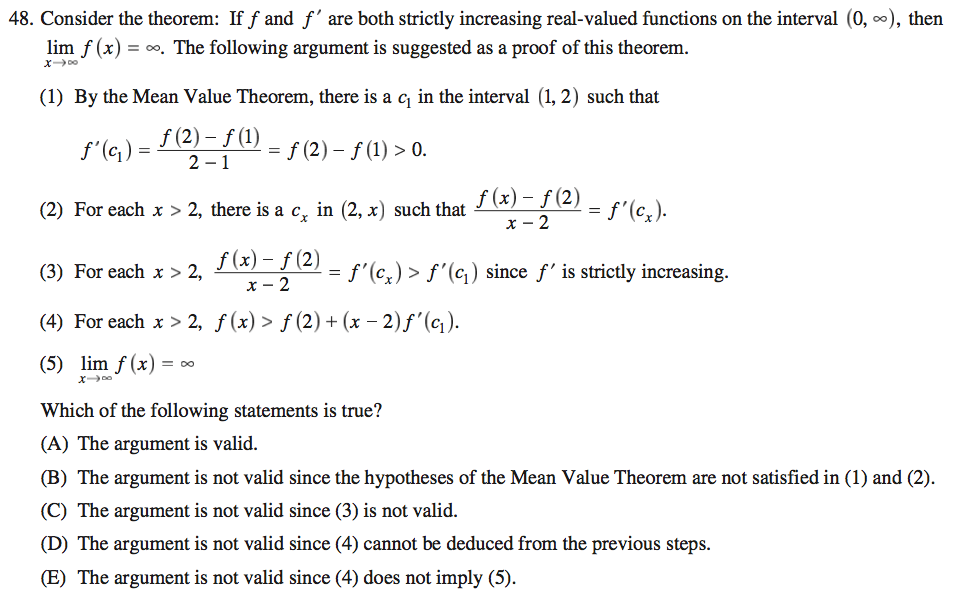
\includegraphics[scale=0.5]{0568_48}

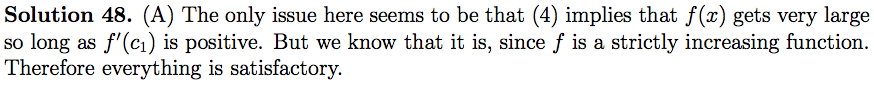
\includegraphics[scale=0.5]{0568_48s}

%\includegraphics[scale=0.65]{1268_53}

%\includegraphics[scale=0.65]{1268_53s}

%\includegraphics[scale=0.65]{1268_55}

%\includegraphics[scale=0.65]{1268_55s}

%\includegraphics[scale=0.65]{1268_56}
%
%\includegraphics[scale=0.65]{1268_56s1}

%\includegraphics[scale=0.65]{1268_56s2}

%\includegraphics[scale=0.65]{1268_64}
%
%\includegraphics[scale=0.65]{1268_64s}

\textbf{Line integrals chapter!} http://tutorial.math.lamar.edu/Classes/CalcIII/LineIntegralsIntro.aspx

\textbf{Surface inegrals chapter!} http://tutorial.math.lamar.edu/Classes/CalcIII/SurfaceIntegralsIntro.aspx

\pagebreak

% Differential Equations
\section{Differential Equations}

\includegraphics[scale=0.65]{1268_61}

\includegraphics[scale=0.65]{1268_61s}

\pagebreak

% Real Analysis
\section{Real Analysis}

\textbf{Brush up on recent real analysis (especially open, closed, compact, etc)}

%\includegraphics[scale=0.65]{1268_36}
%
%\includegraphics[scale=0.65]{1268_36s}

\includegraphics[scale=0.5]{0568_38}

\includegraphics[scale=0.5]{0568_38s}

\includegraphics[scale=0.65]{1268_47}

\includegraphics[scale=0.65]{1268_47s}

\includegraphics[scale=0.65]{1268_57}

\includegraphics[scale=0.65]{1268_57s}

\includegraphics[scale=0.65]{1268_60}

\includegraphics[scale=0.65]{1268_60s}

\includegraphics[scale=0.65]{1268_63}

\includegraphics[scale=0.65]{1268_63s}

\pagebreak

% Probability

\section{Probability}

\subsection{To Know for Math 505A Midterm 1 (Discrete Random Variables)}

\subsubsection{Definitions}

The \textbf{probability mass function} of a discrete random variable \(X\) is the function \(f: \mathbb{R} \to [0,1]\) given by \(f(x) = \Pr(X = x)\).

The \textbf{(cumulative) distribution function} of a discrete random variable \(F\) is given by \[F(x) = \sum_{i:x_i \leq x} f(x_i)\]

The \textbf{joint probability mass function} \(f: \mathbb{R}^2 \to [0, 1]\) of two discrete random variables \(X\) and \(Y\) is given by

\[
f(x, y) = \Pr(X = x \cap Y = y)
\]

The \textbf{joint distribution function} \(F: \mathbb{R}^2 \to [0, 1]\) is given by

\[
F(x, y) = \Pr(X \leq x \cap Y \leq y)
\]

If \(\Pr(B) > 0\) then the \textbf{conditional probability} that \(A\) occurs given that \(B\) occurs is defined to be

\[
\Pr(A \mid B) = \frac{\Pr(A \cap B)}{\Pr(B)}
\]

If \(X\) is a random variable and \(Y\) is a discrete random variable taking on values \(y_1, y_2, \ldots, y_n\), then \(\Pr(X) = \sum_i \Pr(X \mid Y = y_i) \cdot \Pr(Y = y_i)\). (Can be used to prove independence.)

Two random variables \(X\) and \(Y\) are \textbf{uncorrelated} if \(\E(XY) = \E(X) \E(Y)\). Two random variables are uncorrelated if and only if their covariance \(\Cov(X, Y) = \E \big[(X - \E(X))(Y - \E(Y))\big] = \E(XY) - \E(X)\E(Y)\)  equals 0. If \(X\) and \(Y\) are independent then the are uncorrelated.

Two random variables \(X\) and \(Y\) are \textbf{independent} if and only if \(\Pr(X \cap Y) = \Pr(X) \Pr(Y)\).

\textbf{Thereom.} If \(X\) and \(Y\) are independent and \(g, h: \mathbb{R} \to \mathbb{R}\), then \(g(X)\) and \(h(Y)\) are also independent.

\subsubsection{Conditioning}

The \textbf{conditional distribution function} of \(Y\) given \(X = x\), written \(F_{Y\mid X}( \cdot \mid x)\), is defined by

\[
F_{Y\mid X}( y \mid x) = \Pr(Y \leq y \mid X = x)
\]

The \textbf{conditional probability mass function} of \(Y\) given \(X = x\), written \(f_{Y\mid X}( \cdot \mid x)\), is defined by

\[
f_{Y\mid X}( y \mid x) = \Pr(Y = y \mid X = x)
\]

\textbf{Iterated expecations:} 

\begin{itemize}

\item \(\E\big[ \E(Y \mid X) \big] = \E(Y)\)

\item \(\E \big[ (X \mid Y) \mid Z \big] = \E(X \mid Y)\)

\end{itemize}

\textbf{Conditional Variance:} \(\Var(X \mid Y) = \E\big[ (X - \E(X \mid Y))^2   \mid Y\big]\)

\subsubsection{Odds and Ends}

\textbf{Sums of random variables.} If \(X\) and \(Y\) are independent then

\[
\Pr(X + Y = z) = f_{X +Y}(z) = \sum_x f_X(x) f_Y(z-x) = \sum_y f_X(z - y) f_Y(y)
\]

\textbf{Variance-Covariance Expansion.} Let \(X_1, \ldots, X_n\) be random variables. If \(\E \left|X_k \right|^2 < \infty\), then 

\[
\Var(X_1 + \ldots + X_n) = \sum_k \Var(X_k) + \sum_{k \neq m} \sum_m \Cov(X_k, X_m)
\]

\subsubsection{Methods for Calculating Quantities}

\begin{itemize}

\item Expectation

\begin{itemize}

\item Definition: \(\E(X) = \sum_x x \Pr(X = x)\)\

\item Useful theorems: \(\E(aX + bY) = a \E(X) + b \E(Y)\); if \(X \geq 0\) then \(\E(X) \geq 0\).

\item \textbf{Law of the Unconscious Statistician:} If \(X\) has mass function \(f\), and \(g: \mathbb{R} \to \mathbb{R}\), then 

\[
\E(g(X)) = \sum_x g(x) f(x)
\]

\item Expectation is a linear operator: \( \E \big(\sum_i X_i \big) = \sum_i \E(X_i)\)



\end{itemize}

\item Variance

\begin{itemize}

\item Definition: \( \Var(X) = \E(X - \E(X))^2\)

\item Useful reformulation: \(\Var(X) = \E(X^2) - \E(X)^2\)

\item Useful theorems: \(\Var(aX) = a^2 \Var(X)\), \(\Var(X + Y) = \Var(X) + \Var(Y) + 2 \Cov(X, Y)\), \(\Var(aX \pm bY) = a^2\Var(X) + b^2\Var(Y) \pm 2ab \Cov(X, Y)\)

\item \textbf{Total variance:} \( \Var(X) = \Var \big( \E(X \mid Y) \big) + \E \big( \Var(X \mid Y) \big) \)

\end{itemize}

\item Covariance

\begin{itemize}

\item Definition: \( \Cov(X, Y ) = \E \big[ (X - \E(X))(Y - \E(Y))\big] \)

\item Useful reformulation: \(\Cov(X) = \E(XY) - \E(X)\E(Y)\)

\end{itemize}

\end{itemize}

\subsubsection{Discrete Random Variable Distributions}

\textbf{Binomial}: \(\operatorname{Binomial}(n, p)\) (sum of \(n\) Bernoulli random variables)

\begin{itemize}

\item Mass function: \(\Pr(X = k) = \binom{n}{k}p^k(1-p)^{n-k}  \)

\item Distribution: \(\Pr(X \leq k) = \sum_{i=0}^k \binom{n}{i}p^i(1-p)^{n-i} \)

\item Expectation: \(\E(X) = np \)

\item Variance: \(\Var(X) = np(1-p) \)

\end{itemize}

\textbf{Poisson}:  \(\operatorname{Poisson}(\lambda)\): an approximation of the binomial distribution for n very large, p very small, \(np \to \lambda \in (0, \infty)\).

\begin{itemize}

\item Mass function: \[\Pr(X = k) =  \frac{e^{-\lambda}\lambda^k}{k!} \]

\item Distribution: \(\Pr(X \leq k) = \sum{i=0}^k  \frac{e^{-\lambda}\lambda^i}{i!}  \)

\item Expectation: \(\E(X) = \lambda \) (derive from basic definitions)

\item Variance: \(\Var(X) = \lambda\)

\end{itemize}

\textbf{Geometric}:  \(\operatorname{G}_1(p)\): the number of Bernoulli trials before the first success.

\begin{itemize}

\item Mass function: \(\Pr(X = k) = p(1-p)^{k-1} \)

\item Distribution: \(\Pr(X \leq k) = \sum_{i=1}^k p(1-p)^{k-1}  \)

\item Expectation: \(\E(X) = 1/p \)

\item Variance: \(\Var(X) = (1-p)/p^2\)

\end{itemize}


\textbf{Negative binomial}: \( \operatorname{NB}(r, p)\): The number of Bernoulli trials required for \(r\) successes. (Can be derived as the sum of \(r\) identically distributed geometric random variables.)

\begin{itemize}

\item Mass function: \(\Pr(X = k) =  \binom{k-1}{r-1} p^r (1-p)^{k-r}\)

\item Distribution: \(\Pr(X \leq k) = \sum_{i=r}^k \binom{i-1}{r-1} p^r (1-p)^{i-r} \)

\item Expectation: \(\E(X) = \)

\item Variance: \(\Var(X) = \)

\end{itemize}


\textbf{Hypergeometric}: \( \operatorname{Hypergeometric}(N, M, K)\): When drawing a sample of size \(K\) from a group of \(N\) items, \(M\) of which are special, the number of special items retrieved.

\begin{itemize}

\item Mass function: \[\Pr(X = k) = \frac{\binom{M}{k} \binom{N-M}{K-k}}{\binom{N}{K}} \]

\item Distribution: \[\Pr(X \leq k) = \sum_{i=0}^k \frac{\binom{M}{i} \binom{N-M}{K-i}}{\binom{N}{K}}  \]

\item Expectation: \(\E(X) = \) (find by indicator method)

\item Variance: \(\Var(X) = \) (find by indicator method)

\end{itemize}


\subsubsection{Indicator Method}

If \(\boldsymbol{1}_{A_k}\) is an indicator then

\[
\Cov(\boldsymbol{1}_{A_k}, \boldsymbol{1}_{A_m}) = \E(\boldsymbol{1}_{A_k} \boldsymbol{1}_{A_m}) - \E(\boldsymbol{1}_{A_k}) \E(\boldsymbol{1}_{A_m}) = \Pr(A_k \cap A_m) - \Pr(A_k) \Pr(A_m)
\]

\[
\Var(\boldsymbol{1}_{A_k} ) = \E(\boldsymbol{1}_{A_k} ^2) = \E(\boldsymbol{1}_{A_k} )^2 = \Pr(A_k) - (\Pr(A_k))^2
\]

Example problems: 505A Homework 3 problem 9(a)

Worked examples in p. 56 - 59 of Grimmet and Stirkazer 3rd edition.

\subsubsection{Linear transformations of random variables}

\subsubsection{Poisson Paradigm (Poisson approximation for indicator method)}

(Theorem 9, p. 129.) Let \(A_i\) be an event. If \(X = \sum_{i=1}^m \boldsymbol{1}_{A_i}\) where \(\boldsymbol{1}_{A_i}\) is an indicator variable for \(A_i\), and the \(A_i\) are only weakly dependent on each other, then 

\[
\text{As } m \to \infty, \ \ X \sim \operatorname{Poisson}(\E(X))
\]

More specifically, let \(B_i\) be \(n\) independent Bernoulli random variables with probabilities \(p_i\). If \(Y = \sum_{i=1}^n B_i\) then 

\[
\text{As } n \to \infty, \ \ Y \sim \operatorname{Poisson} \bigg(\E \bigg(\sum_i B_i \bigg) \bigg) = \operatorname{Poisson}\bigg(\sum_i \E B_i \bigg) = \operatorname{Poisson}\bigg(\sum_i p_i \bigg) 
\]

\subsubsection{Asymptotic Distributions}

\[
e^x = \lim_{n \to \infty} \bigg( 1 + \frac{x}{n}\bigg)^n
\]

\textbf{Stirling's Formula}: 

\[
n! \approx n^ne^{-n} \sqrt{2\pi n}
\]

\subsubsection{Example Problems That Will Likely Appear on Midterm}

\textbf{Fall 2014 Problem 1 (likely to be question 2 on the midterm).} Let \(A\) and \(B\) be two events with \(0 < \Pr(A) < 1, \ 0 < \Pr(B) < 1\). Define the random variables \(\xi = \xi(\omega)\) and \(\eta = \eta(\omega)\) by

\[
\xi(\omega) = \begin{cases} 
      5 & \text{ if } \omega \in A \\
      -7 &  \text{ if } \omega \notin A 
   \end{cases}, \ \ \ \ \eta(\omega) = \begin{cases} 
      2 & \text{ if } \omega \in B \\
      3 &  \text{ if } \omega \notin B 
   \end{cases}
\]

True or false: the events \(A\) and \(B\) are independent if and only if the random variables \(\xi\) and \(\eta\) are uncorrelated?

\textbf{Solution.} (\(\implies\)) Suppose \(A\) and \(B\) are independent. Then \(\xi\) and \(\eta\) are uncorrelated if and only if \(\E(\xi \eta ) = \E(\xi) \E(\eta)\). We can write \(\xi = 5 \cdot \boldsymbol{1}_A - 7 \cdot \boldsymbol{1}_{A^c}\) and \(\eta = 2 \cdot \boldsymbol{1}_B + 3 \cdot \boldsymbol{1}_{B^c}\). So we have

\[
\xi \eta = (5 \cdot \boldsymbol{1}_A - 7 \cdot \boldsymbol{1}_{A^c})(2 \cdot \boldsymbol{1}_B + 3 \cdot \boldsymbol{1}_{B^c}) = 10 \cdot \boldsymbol{1}_{A \cap B} +15 \cdot \boldsymbol{1}_{A \cap B^c} - 14 \cdot \boldsymbol{1}_{A^c \cap B} - 21 \cdot \boldsymbol{1}_{A^c \cap B^c}
\]

\[
\implies \E(\xi \eta ) = 10 \Pr(A \cap B) +15\Pr(A \cap B^c) - 14 \Pr(A^c \cap B) - 21\Pr(A^c \cap B^c)
\]

Then

\[
\E(\xi) \E(\eta) = (5 \Pr(A) - 7 \Pr(A^c))(2 \Pr(B) + 3 \Pr(B^c)) 
\]

\[
= 10\Pr(A \cap B) + 15 \Pr(A \cap B^c) - 14 \Pr(A^c \cap B) - 21 \Pr(A^c \cap B^c) = \E(\xi \eta )
\]

where the second-to-last step follows from the independence of \(A\) and \(B\). Therefore \(\eta\) and \(\xi\) are uncorrelated.

(\(\impliedby\)) Now suppose \(\eta\) and \(\xi\) are uncorrelated. Then \(\xi\) and \(\eta\) are independent if and only if \(\Pr(\xi \cap \eta) = \Pr(\xi) \Pr(\eta)\). Define

\[
\alpha(\omega) =  \xi(\omega) + 7 = \begin{cases} 
      12 & \text{ if } \omega \in A \\
      0 &  \text{ if } \omega \notin A 
   \end{cases}, \ \ \ \ \beta(\omega) =  \eta(\omega) - 3 = \begin{cases} 
      -1 & \text{ if } \omega \in B \\
      0 &  \text{ if } \omega \notin B 
   \end{cases}
\]

Then we have

\[
(\alpha \beta)(\omega) = \begin{cases} 
      -12 & \text{ if } \omega \in A \cap B \\
      0 &  \text{ otherwise} 
   \end{cases}
\]

Then

\[
\E(\xi \eta) = \E\big[ (\alpha - 7)(\beta + 3)\big] = \E(\alpha \beta) + 3 \E(\alpha) - 7 \E(\beta) - 21
\]

\[
\E(\xi) \E(\eta) = (\E(\alpha) - 7) (\E(\beta) + 3) = \E(\alpha) \E(\beta) - 7 \E(\beta) + 3 \E(\alpha) - 21
\]

Since by assumption \( \E(\xi \eta)  = \E(\xi) \E(\eta) \), this yields \(\E(\alpha \beta) = \E(\alpha) \E(\beta) \). But

\[
\E(\alpha \beta) = -12 \Pr(A \cap B), \ \ \ \ \ \E(\alpha) \E(\beta) = 12 \Pr(A) (-1) \Pr(B) = -12\Pr(A)\Pr(B)
\]

Therefore \(\Pr(\xi \cap \eta) = \Pr(\xi) \Pr(\eta)\) and \(\xi\) and \(\eta\) are independent.

\textbf{Fall 2009 Problem 4 (Very similar).} Let \(X\) and \(Y\) be two random variables, both taking only two values. Show that if they are uncorrelated, then they are independent.

\textbf{Solution.} Let \(X\) and \(Y\) have the following pmfs: \(\Pr(X = a) = p, \Pr(X = b) = 1-p; \ \ \ \Pr(Y = c) = q, \Pr(Y = d) = 1  -q \). Suppose \(X\) and \(Y\) are uncorrelated; that is, \(\E(XY) = \E(X)\E(Y)\). Then \(X\) and \(Y\) are independent if \(\Pr(X \cap Y) = \Pr(X) \Pr(Y)\). Since these random variables take on only two values each, this can also be expressed as \( \Pr(X = a \cap Y = c) = \Pr(X = a) \Pr(Y = c)\). 

Begin by defining new variables \(\alpha = X - b\) and \(\beta = Y - d\). Then we have

\[
\E(\alpha \beta) = \E( (X - b)(Y - d)) = \E(XY) - b \E(Y) -d \E(X) + bd
\]

\[
\E(\alpha) \E(\beta) = \E(X-b) \E(Y - d) = \E(X)\E(Y) -b \E(Y) -d \E(X) + bd
\]

Since by assumption \(\E(XY) = \E(X)\E(Y)\), this yields \(\E(\alpha \beta)  = \E(\alpha) \E(\beta) \). But \(\E(\alpha) = p(a-b) = (a - b) \Pr(X = a)\), \(\E(\beta) = q(c-d) = (c -d) \Pr(Y = c)\), \(\E(\alpha \beta) = (a-b)(c-d)pq = (a - b)(c - d) \Pr(X = a \cap Y = c)\). Therefore

\[
\E(\alpha \beta)  = \E(\alpha) \E(\beta)  \iff  (a - b)(c - d) \Pr(X = a \cap Y = c) = (a - b) \Pr(X = a) (c -d) \Pr(Y = c)
\]

\[
\iff \Pr(X = a \cap Y = c) = \Pr(X = a)  \Pr(Y = c)
\]

which proves the independence of \(X\) and \(Y\).

\textbf{Fall 2011 Problem 1 (same as HW1 problem 5; similar to HW3 problem 2(5); likely to be question 1 on the midterm.)} True or false: if \(A\) and \(B\) are events such that \( 0 < \Pr(A) < 1\) and \(\Pr(B \mid A) = \Pr(B \mid A^c)\), then \(A\) and \(B\) are independent.

\textbf{Solution.} \(A\) and \(B\) are independent if and only if 

\[
\Pr(A \cap B) = \Pr(A)\cdot\Pr(B)
\]

We know that \[ \Pr(B) = \Pr(B|A)\cdot \Pr(A) + \Pr(B|A^c)\cdot\Pr(A^c)  \]

\[
= \Pr(B|A)\cdot \Pr(A) + \Pr(B|A)\cdot (1 - \Pr(A)) = \Pr(B|A)\cdot \Pr(A) + \Pr(B|A) - \Pr(B|A)\cdot \Pr(A) 
\]

\[
= \Pr(B|A)
\]

Also, we know that since \(\Pr(A) \neq 0\),

\[
\Pr(B|A) = \frac{\Pr(A \cap B)}{\Pr(A)} 
\]

Per above \(\Pr(B|A) = \Pr(B)\), so we have

\[
\Pr(B) = \frac{\Pr(A \cap B)}{\Pr(A)} 
\]

\[
\Pr(A \cap B)= \Pr(A) \cdot \Pr(B)
\]

which is what we were trying to prove. So the answer is \(\boxed{\text{true.}}\)

\textbf{Similar problem: HW3 Problem 2(5).}

\textbf{Fall 2008 Problem 2 (HW1 Problem 10)}

\textbf{HW1 Problem 8}

\subsubsection{Problems we did in class that professor mentioned}

\textbf{Spring 2018 Problem 2}

\textbf{Variance Problem 09/21}

\textbf{Independence Problem 09/24}

\subsubsection{Problems we did on homework}

\textbf{Fall 2017 Problem 2/Fall 2009 Problem 1 (HW3 Problem 6)}

\textbf{Fall 2017 Problem 3 (HW3 Problem 8)}

\textbf{Spring 2016 Problem 3 (HW3 Problem 5)}

\textbf{Fall 2013 Problem 3/Spring 2011 Problem 2 (HW3 Problem 9; coupon collector problem)}

\textbf{Fall 2012 Problem 1 (HW2 Problem 10/HW 1 Problem 9)}

\subsection{To Know for Math 505A Midterm 2}

\subsubsection{Definitions}

A \textbf{probability density function} for a continuous random variable 

A \textbf{cumulative distribution function} or \textbf{distribution} of a continuous random variable

\subsubsection{Inequalities}

\pagebreak

% Abstract Algebra

\section{Abstract Algebra}

These are my notes from reading \textit{Elementary Abstract Algebra} by W. Edwin Clark, available for free download on his website: \url{http://shell.cas.usf.edu/~wclark/#ELEMENTARY_ABSTRACT_ALGEBRA}

% Chapter 1
\subsection{Chapter 1: Binary Operations}

\includegraphics[scale=0.65]{binary_operation}

%\includegraphics[scale=0.45]{function}

\textbf{Definition:} A \textbf{function} \(f\) from the set \(A\) to the set \(B\) is a rule which assigns to each element \(a \in A\) an element \(f(a) \in B\) in such a way that the following condition holds for all \(x, y \in A\):

\[
x = y \implies f(x) = f(y)
\]

To indicate that \(f\) is a function from \(A\) to \(B\) we write \(f: A \to B\). The set \(A\) is called the \textbf{domain} of \(f\) and the set \(B\) is called the \textbf{codomain} of \(f\).

%\includegraphics[scale=0.45]{onto}

A function \(f: A \to B\) is said to be \textbf{one-to-one} or \textbf{injective} if the following condition holds for all \(x, y \in A\):

\[
f(x) = f(y) \implies x = y
\]

A function \(f: A \to B\) is said to be \textbf{onto} or \textbf{surjective} if the following condition holds:

\[
\forall \ b \in B \ \exists \ a \in A \ | \ f(a) = b
\]

A function \(f: A \to B\) is said to be \textbf{bijective} if it is both one-to-one and onto. Then \(f\) is sometimes said to be a \textbf{bijection} or a \textbf{one-to-one correspondence} between \(A\) and \(B\).

\includegraphics[scale=0.65]{1268_15}

\includegraphics[scale=0.65]{1268_15s}

Let \(S\) be a set. The \textbf{power set} \(\mathcal{P}(S)\) of \(S\) is the set of all subsets of \(S\) (including \(S\) itself).

\includegraphics[scale=0.45]{binary_operation2}

\pagebreak

For each integer \(n \geq 2\) define the set

\[
\mathbb{Z}_n = \{0, 1, 2, \ldots, n-1\}
\]

For all \(a, b \in \mathbb{Z}_n\) let \[a + b = \text{remainder when the ordinary sum of a and b is divided by n}\] and \[a \cdot b = \text{remainder when the ordinary product of a and b is divided by n.}\]

These binary operations are referred to as \textbf{addition modulo \(n\)} and \textbf{multiplication modulo \(n\)}. The integer \(n\) in \(\mathbb{Z}_n\) is called the \textbf{modulus}. The plural of modulus is \textbf{moduli}.

Let \(K\) denote any one of the following: \(\mathbb{Z}, \mathbb{Q}, \mathbb{R}, \mathbb{Z}_n\). \[M_n(K)\] is the set of all \(n \times n\) matrices containing elements of \(K\). \[GL(n, K)\] is the set of all matrices in \(M_{n}(K)\) with non-zero determinant. \((GL(n, k), \cdot)\) is called the \textbf{general linear group of degree n over K}. It is non-abelian.

\[
SL(n, K) = \{A \in GL(n, K) \ | \ \det(A) = 1\}
\]

\(SL(n, K)\) is called the \textbf{Special Linear Group of degree \(n\) over \(K\)}.

\pagebreak

% Chapter 2
\subsection{Chapter 2: Groups}

\textbf{Definition} A \textbf{group} is an ordered pair \((G, *)\) where \(G\) is a set and \(*\) is a binary operation on \(G\) satisfying the following properties:

\begin{enumerate}[1.]

\item \textbf{The binary operation is associative on \(G\):} \(\forall \ x, y , z \in G\), 

\[
x * (y * z) = (x * y) * z
\]

\item \textbf{The binary operation contains a (unique) identity in \(G\):} \(\exists \ e \in G \ | \ \forall \ x  \in  G\)

\[
e * x = x, \ x * e = x 
\]

\item \textbf{Every element in \(G\) has a (unique) inverse on \(*\) in \(G\):} \(\forall \ x \in G \ \exists \ y \in G \ |\)

\[
x*y = e, y*x =e
\]

A group \( (G, *)\) is said to be \textbf{abelian} if \(\forall \ x, y \in G, \ x*y = y*x\). A group is said to be \textbf{non-abelian} if it is not abelian.

\end{enumerate}

\includegraphics[scale=0.45]{group_properties}

\pagebreak
% Chapter 3
\subsection{Chapter 3: The Symmetric Groups}

If \(n\) is a positive integer, \[[n] = \{ 1, 2, \ldots, n \} \] A \textbf{permutation} of \([n]\) is a one-to-one, onto function from \([n]\) to \([n]\), and \[S_n\] is the set of all permutations of \([n]\).

The identity of \(S_n\) is the so-called \textbf{identity function}

\[
\iota : [n] \to [n]
\]

which is defined by the rule

\[
\iota(x) = x, \ \ \forall \ x \in [n]
\]

\textbf{The inverse of an element \(\sigma \in S_n\):} Suppose \(\sigma \in S_n\). Since \(\sigma\) is by definition one-to-one and onto, the rule

\[
\sigma^{-1}(y) = x \iff \sigma(x) = y
\]

defines a function \(\sigma^{-1}: [n] \to [n]\). This function \(\sigma^{-1}\) is also one-to-one and onto and satisfies

\[
\sigma \sigma^{-1} = \iota \text{       and         } \sigma^{-1}\sigma = \iota
\]

so it is the inverse of \(\sigma\) in the group sense also.

Since the binary operation of composition on \(S_n\) is associative [\(  (\gamma \beta) \alpha = \gamma (\beta \alpha)  \)], \(S_n\) under the binary operation of composition is a group (it is associative, it has an inverse, and it has an identity).

\includegraphics[scale=0.45]{cycle}

Two cycles \((i_1 \ i_2 \ \ldots \ i_k)\) and \((j_1 \ j_2 \ \ldots \ j_l)\) are said to be \textbf{disjoint} if the sets \(\{i_1, i_2, \ldots, i_k\}\) and \(\{j_1, j_2, \ldots, j_l\}\) are disjoint.

So for example, the cycles \((1 \ 2 \ 3)\) and \((4 \ 5 \ 8)\) are disjoint, but the cycles \((1 \ 2 \ 3)\) and \((4 \ 2 \ 8)\) are not disjoint.

If \(\sigma\) and \(\tau\) are disjoint cycles, then \(\sigma \tau = \tau \sigma\).

\includegraphics[scale=0.45]{disjoint_cycle_decomp}

An element of \(S_n\) is called a \textbf{transposition} if and only if it is a 2-cycle. 

Every element of \(S_n\) can be written as a product of transpositions. The factors of such a product are not unique. However, if \(\sigma \in S_n\) can be written as a product of \(k\) transpositions and if the same \(\sigma\) can also be written as a product of \(l\) transpositions, then \(k\) and \(l\) have the same parity.

A permutation is \textbf{even} if it is a product of an even number of transpositions and \textbf{odd} if it is a product of an odd number of transpositions. We define the function \(\text{sign} : S_n \to \{1, -1\}\) by 

\[
\text{sign}(\sigma) = \begin{cases} 
     1 & \text{if } \sigma \text{ is even} \\
     -1 & \text{if } \sigma \text{ is odd}
   \end{cases}
\]

If \(n = 1\) then there are no transpositions. In this case, to be complete we define the identity permutation \(\iota\) to be even.

If \(\sigma\) is a \(k\)-cycle, then \(\text{sign}(\sigma) = 1\) if \(k\) is odd and \(\text{sign}(\sigma) = -1\) if \(k\) is even.

\includegraphics[scale=0.45]{determinant}

\textbf{Definition:} If \((G, *)\) is a group, the number of elements in \(G\) is called the \textbf{order} of \(G\). We use \(|G|\) to denote the order of \(G\). Note that \(|G|\) may be finite or infinite.

Let \[A_n\] be the set of all even permutations in the group \(S_n\). \(A_n\) is called the \textbf{alternating group of degree \(n\)}.

\pagebreak
% Chapter 4
\subsection{Chapter 4: Subgroups}

\textbf{Definition:} Let \(G\) be a group. A \textbf{subgroup} of \(G\) is a subset \(H\) of \(G\) which satisfies the following three conditions:


\begin{enumerate}[1.]

\item \(e \in H\)

\item \(a, b \in H \implies ab \in H\)

\item \(a \in H \implies a^{-1} \in H\)

\end{enumerate}


If \(H\) is a subgroup of \(G\), we write \(H \leq G\). The subgroups \(\{e\}\) and \(G\) are said to be \textbf{trivial} subgroups of \(G\).

Every finite subgroup may be thought of as a subgroup of one of the groups \(S_n\).

Let \(A_n\) be the set of all even permutations in the group \(S_n\). \(A_n\) is then a subgroup of \(S_n\). \(A_n\) is called the \textbf{alternating group of degree \(n\)}.

Let \(a\) be an element of the group \(G\). If \(\exists \ n \in \mathbb{N} \ | \ a^n = e\) we say that \(a\) has \textbf{finite order} and we define

\[
\text{o}(a) = \min \{n \in \mathbb{N} \ | \ a^n = e\}
\]

If \(a^n \neq e \ \forall \ n \in \mathbb{N}\) we say that \(a\) has \textbf{infinite order} and we define

\[
\text{o}(a) = \infty
\]

In either case we call \(\text{o}(a)\) the \textbf{order} of \(a\). Note carefully the difference between the order of a group and the order of an element of a group. Note also that \(a = e \iff \text{o}(a) = 1\). So every element of a group other than \(e\) has order \(n \geq 2\) or \(\infty\).

Let \(a\) be an element of group \(G\). Define

\[
\langle a \rangle = \{a^i  : i \in \mathbb{Z} \}
\]

We call \(\langle a \rangle\) the \textbf{subgroup of \(G\) generated by \(a\)}. Note that \(e = a^0\) and \(a^{-1}\) are in \(\langle a \rangle\).

\textbf{Theorem.} For each \(a \in G\), \(\langle a \rangle\) is a subgroup of \(G\). \(\langle a \rangle\) contains \(a\) and is the smallest subgroup of \(G\) containing \(a\). 

\textbf{Proof of second statement.} If \(H\) is any subgroup of \(G\) containing \(a\), \(\langle a \rangle \subseteq H \) since \(H\) is closed under taking products and inverses. That is, every subgroup of \(G\) containing \(a\) also contains \(\langle a \rangle\). This implies that \(\langle a \rangle\) is the smallest subgroup of \(G\) containing \(a\).

\pagebreak 
\textbf{Theorem.} Let \(G\) be a group and let \(a \in G\). If \(\text{o}(a) = 1\), then \(\langle a \rangle = \{e \}\). If \(\text{o}(a) = n\) where \(n \geq 2\), then

\[
\langle a \rangle = \{e, a, a^2, \ldots, a^{n-1} \}
\]

and the elements \(e, a, a^2, \ldots, a^{n-1}\) are distinct; that is, 

\[
\text{o}(a) = | \langle a \rangle |
\]

\includegraphics[scale=0.4]{ch4_proof}

\textbf{Theorem.} If \(G\) is a finite group, then every element of \(G\) has finite order.

\includegraphics[scale=0.65]{1268_49}

\includegraphics[scale=0.65]{1268_49s}

\pagebreak
% Chapter 5
\subsection{Chapter 5: The Group of Units of \(\mathbb{Z}_n\)}

Let \(n \geq 2\). An element \(a \in \mathbb{Z}_n\) is said to be a \textbf{unit} if \(\exists \ b \in \mathbb{Z}_n \ | \ ab = 1\) (where the product is multiplication modulo \(n\)). 

The set of all units in \(\mathbb{Z}_n\) is denoted by \[U_n\] and is a group under multiplication modulo \(n\) called the \textbf{group of units of \(\mathbb{Z}_n\)}.

\textbf{Theorem.} For \(n \geq 2 \), \(U_n = \{a \in \mathbb{Z}_n: \gcd(a, n) = 1 \} \)

\textbf{Theorem.} \(p\) is a prime \(\implies \exists \ a \in U_p \ | \ U_p = \langle a \rangle\)

\textbf{Theorem.} If \(n \geq 2\) then \(U_n\) contains an element \(a\) satisfying \(U_n = \langle a \rangle\) if and only if \(a\) has one of the following forms: \(2, \ 4, \ p^k\), or \(2p^k\) where \(p\) is an odd prime and \(k \in \mathbb{N}\).

%\pagebreak
% Chapter 6
\subsection{Chapter 6: Direct Products of Groups}

If \(G_1, G_2, \ldots, G_n\) is a list of \(n\) groups we make the Cartesian product \(G_1 \times G_2 \times \cdots \times G_n\) into a group by defining the binary operation

\[
(a_1, a_2, \ldots, a_n) \cdot (b_1, b_2, \ldots, b_n) = (a_1 \cdot b_1, a_2 \cdot b_2, \ldots, a_n \cdot b_n)
\]

Here for each \(i \in \{1, 2, \ldots, n\}\) the product \(a_i \cdot b_i\) is the product of \(a_i\) and \(b_i\) in the group \(G_i\). We call this group the \textbf{direct product} of the groups \(G_1, G_2, \ldots, G_n\).

The direct product contains an identity and an inverse, and is associative (since it is composed of groups which must themselves be associative), so it is a group per below:

\textbf{Theorem.} If \(G_1, G_2, \ldots, G_n\) is a list of \(n\) groups, the direct product \(G = G_1 \times G_2 \times \cdots \times G_n\) as defined above is a group. Moreover, if for each \(i\), \(e_i\) is the identity of \(G_i\), then \(e_1, e_2, \ldots, e_n\) is the identity of \(G\), and if 

\[
\boldsymbol{a} = (a_1, a_2, \ldots, a_n) \in G
\]

then the inverse of \(\boldsymbol{a}\) is given by

\[
\boldsymbol{a}^{-1} = (a_1^{-1}, a_2^{-1}, \ldots, a_n^{-1})
\]

where \(a_i^{-1}\) is the inverse of \(a_i\) in the group \(G_i\).

\pagebreak
% Chapter 7
\subsection{Chapter 7: Isomorphism of Groups}

Let \(G = \{g_1, g_2, \ldots, g_n \}\). Let \(\text{o}(g_i) = k_i\) for \(i = 1, 2 , \ldots, n\). We say that the sequence \((k_1, k_2, \ldots, k_m) \) is the \textbf{order sequence} of the group \(G\). To make the sequence unique we assume the elements are ordered so that \(k_1 \leq k_2 \leq \ldots \leq k_n\).

Let \((G, *)\) and \((H, \bullet)\)  be groups. A function \(f : G \to H\) is said to be a \textbf{homomorphism} from \(G\) to \(H\) if

\[
f(a * b) = f(a) \bullet f(b)
\]

for all \(a, b \in G\). If in addition \(f\) is one-to-one and onto, \(f\) is said to be an \textbf{isomorphism} from \(G\) to \(H\).

We say that \(G\) and \(H\) are \textbf{isomorphic} if and only if there is an isomorphism from \(G\) to \(H\). We write \(G \cong H\) to indicate that \(G\) is isomorphic to \(H\).

\textbf{Isomorphism is an equivalence relation:} If \(G, H\), and \(K\) are groups then

\begin{enumerate}[1.]

\item \(G \cong G\)

\item If \(G \cong H\) then \(H \cong G\), and

\item If \(G \cong H\) and \(H \cong K\), then \(G \cong K\).

\end{enumerate}

\textbf{Theorem.} Let \((G, *)\) and \((H, \bullet)\) be groups and let \(f: G \to H\) be a homomorphism. Let \(e_G\) denote the identity of \(G\), and let \(e_H\) denote the identity of \(H\). Then

\begin{enumerate}[1.]

\item \(f(e_G) = e_H\)

\begin{center}
\textit{Proof: Let \(x_G \in G\) and let \(f(x_G) = x_H \in H\). Then \(x_H = f(x_G) = f(e_G * x_G) = f(e_G) \bullet f(x_G) = f(e_G) \bullet x_H = e_H \bullet x_H\).}
\end{center}

\item \(f(a^{-1}) = f(a)^{-1}\)

\begin{center}
\textit{Proof: \(f(a)^{-1} \bullet f(a) = e_H = f(e_G) = f(a^{-1} * a) = f(a^{-1}) \bullet f(a)\)}
\end{center}

\item \(f(a^n) = f(a)^n \ \forall \ n \in \mathbb{Z}\)

\begin{center}
\textit{Proof by induction.}
\end{center}

\end{enumerate}

\textbf{Theorem.} Let \((G, *)\) and \((H, \bullet)\) be groups and let \(f:G \to H\) be an isomorphism. Then \(\text{o}(a) = \text{o}(f(a)) \ \forall \ a \in G\). It follows that \(G\) and \(H\) have the same number of elements of each possible order.

\textbf{Theorem.} If \(G\) and \(H\) are isomorphic groups, and \(G\) is abelian, then so is \(H\).

\begin{center}
\textit{Proof: Let \(a_G, b_G \in G\) and let \(f(a_G) = a_H \in H, f(b_G) = b_H \in H\). \(a_H \bullet b_H = f(a_G) \bullet f(b_G) = f(a_G * b_G) = f(b_G * a_G) = f(b_G) \bullet f(a_G) = b_H \bullet a_H\).}
\end{center}

A group \(G\) is \textbf{cyclic} if there is an element \(a \in G \ | \ \langle a \rangle = G\). If \(\langle a \rangle = G\) then we say that \(a\) is a \textbf{generator} for \(G\). 

\textbf{Theorem.} If \(G\) and \(H\) are isomorphic groups and \(G\) is cyclic then \(H\) is cyclic.

\textbf{Theorem.} Let \(a\) be an element of group \(G\). 

\begin{enumerate}[1.]

\item \(\text{o}(a) = \infty \implies \langle a \rangle \cong \mathbb{Z}\).

\item \(\text{o}(a) = n \in \mathbb{N} \implies \langle a \rangle \cong \mathbb{Z}_n\)

\end{enumerate}

%\includegraphics[scale=0.4]{cyclic_order_proof1}

%\includegraphics[scale=0.4]{cyclic_order_proof2}

\textbf{Cayley's Theorem.} If \(G\) is a finite group of order \(n\), then there is a subgroup \(H\) of \(S_n\) such that \(G \cong H\).

\includegraphics[scale=0.65]{1268_66}

\includegraphics[scale=0.65]{1268_66s}

\pagebreak
% Chapter 8
\subsection{Chapter 8: Cosets and Lagrange's Theorem}

Let \(G\) be a group and let \(H\) be subgroup of \(G\). For each element \(a\) of \(G\) we define

\[
aH = \{ ah \ | \ h \in H\}
\]

We call \(aH\) the \textbf{coset of \(H\) in \(G\) generated by \(a\)}.

Let \(a, b \in G\). Then

\begin{enumerate}[1.]

\item \(a \in aH\) (since \(H\) must contain an identity; specifically, the identity of \(G\))

\item \(|aH| = |H|\) (since \(ah\) is unique)

\item \(aH \cap bH \neq  \emptyset \implies aH = bH\)

\end{enumerate}

\textbf{Lagrange's Theorem.} If \(G\) is a finite group and \(H \leq G\) then \(|H|\) divides \(|G|\).

Any group of prime order is cyclic; therefore, there is only one such group up to isomorphism.

\includegraphics[scale=0.45]{prime_order}

We say that there are \(k\) \textbf{isomorphism classes of groups of order \(n\)} if there are \(k\) groups \(G_1, G_2, \ldots, G_k\) such that

\begin{enumerate}[1.]

\item if \(i \neq j\) then \(G_i\) and \(G_j\) are not isomorphic, and

\item Every group of order \(n\) is isomorphic to \(G_i\) for some \(i \in \{1, 2, \ldots, k\}\).

\end{enumerate}

This is sometimes expressed by saying that "there are \(k\) groups of order \(n\) up to isomorphism" or that "there are \(k\) non-isomorphic groups of order \(n\)."

\includegraphics[scale=0.65]{1268_12}

\includegraphics[scale=0.65]{1268_12s}

\includegraphics[scale=0.45]{isomorphism_groups_order}

There is only one isomorphism class of groups of order \(n\) if \(n\) is prime. But there are some non-primes that have this property; for example, 15.

\textbf{The Fundamental Theorem of Finite Abelian Groups.} If \(G\) is a finite abelian group of order at least 2, then 

\[
G \cong \mathbb{Z}_{p_1^{n_1}} \times \mathbb{Z}_{p_2^{n_2}} \times \cdots \times \mathbb{Z}_{p_s^{n_s}} 
\]

where for each \(i\), \(p_i\) is a prime and \(n_i\) is a positive integer. Moreover, the prime powers \(p_i^{n_i}\) are unique except for the order of the factors.

If the group \(G\) in the above theorem has order \(n\) then

\[
n = p_1^{n_1}p_2^{n_2} \cdots p_s^{n_2}
\]

\includegraphics[scale=0.45]{isomorphism_groups_order2}

\textbf{Corollary.} For \(n \geq 2\), the number of isomorphism classes of abelian groups of order \(n\) is equal to the number of ways to factor \(n\) as a product of prime powers (where the order of the factors does not count).

%\textbf{Remark:} In number theory it is proven that if \(n = ab\) and \(\gcd(a, b) = 1\) then \(\mathbb{Z}_n \cong \mathbb{Z_a} \times \mathbb{Z_b}\). This is called the \textit{Chinese Remainder Theorem.}

\pagebreak
% Chapter 9
\subsection{Chapter 9: Introduction to Ring Theory}

\includegraphics[scale=0.45]{ring_summary}

\includegraphics[scale=0.65]{1268_23}

\includegraphics[scale=0.65]{1268_23s}

\includegraphics[scale=0.65]{1268_50}

\includegraphics[scale=0.65]{1268_50s}

\includegraphics[scale=0.5]{0568_18}

\includegraphics[scale=0.5]{0568_18s}

\pagebreak

% Miscellaneous
\section{Miscellaneous}

\includegraphics[scale=0.5]{0568_6}

\includegraphics[scale=0.5]{0568_6s}

\includegraphics[scale=0.65]{1268_19}

\includegraphics[scale=0.65]{1268_19s}

\includegraphics[scale=0.65]{1268_28}

\includegraphics[scale=0.65]{1268_28s}

\begin{center}
\includegraphics[scale=0.65]{1268_28fig}
\end{center}

\includegraphics[scale=0.65]{1268_38}

\includegraphics[scale=0.65]{1268_38s}

\includegraphics[scale=0.65]{1268_45}

\includegraphics[scale=0.65]{1268_45s}


\end{document}
